\documentclass[journal]{IEEEtran}
\usepackage{amsmath,amssymb,booktabs,array,graphicx}
\usepackage{tikz,pgfplots}
\usetikzlibrary{arrows.meta,positioning,shapes.geometric,fit}
\usepgfplotslibrary{groupplots,fillbetween}
\pgfplotsset{compat=1.18}
\usepackage[hidelinks]{hyperref}
\newcommand{\E}{\mathbb{E}}
\newcommand{\ind}{\mathbb{I}}
\newcommand{\sg}{\operatorname{sg}}
\newcommand{\mean}{\operatorname{mean}}
\definecolor{navy}{HTML}{204A68}
\definecolor{teal}{HTML}{00857D}
\definecolor{orange}{HTML}{D27A32}
\definecolor{purple}{HTML}{7E5B9B}
\tikzset{box/.style={draw=navy,rounded corners=2pt,align=center,font=\scriptsize,
  fill=navy!4,inner sep=5pt},flow/.style={-{Stealth[length=1.6mm]},thick,draw=navy}}
\title{Interaction-Aware Cooperative Residual Reinforcement Learning for Multi-USV Target Defense}
\author{Manuscript in preparation}
\begin{document}
\maketitle
\begin{abstract}
We investigate interaction-aware cooperative residual reinforcement learning for multi-USV target defense. The policy mechanism conditions each vessel's learned--Boids blending on the concurrent candidate controls of its teammates. The learning mechanism supervises a joint critic with paired closed-loop return differences induced by changing one vessel's current blending coefficient while fixing all other current candidates and coefficients. Subsequent controls follow the same frozen policy on each branch's own state. These mechanisms address policy representation and conditional value learning within the original residual control framework. Previous learning runs have not established stable task gains, but that outcome does not establish an expressive limitation of the blending action space. The current investigation therefore tests executable fusion opportunities, the additional information supplied by candidate relations, conditional-value accuracy, and the actor's use of that value. Separately, a predictive pursuit--guard controller captured all 512 intruders across two frozen six-defender banks without breaches or collisions. A first structured composition-student test did not retain that advantage. Predictive results remain a strong reference and diagnostic resource; they do not establish either the original learning mechanism's benefit or the necessity of a hierarchical replacement.
\end{abstract}
\begin{IEEEkeywords}
Multi-robot systems, unmanned surface vehicles, cooperative residual reinforcement learning, candidate-control interaction, conditional value learning.
\end{IEEEkeywords}

\section{Introduction}
Multi-USV defense against an agile intruder requires coordination of heterogeneous control sources. ARBoids~\cite{tao} already adapts the mixture of learned and Boids control using individual observations and teammate relative states. We study two more specific questions: whether explicitly representing concurrent candidate-control relationships improves cooperative blending, and whether intervention-based conditional-value supervision helps the actor choose those blends.

Marine autonomy connects perception, decision making, and control~\cite{qiao}. Territory guarding, distributed pursuit, reach--avoid games, and faster-evader pursuit provide complementary formulations~\cite{fu,chen,yan,fang}; vessel dynamics and shared space couple individual maneuvers~\cite{guo,zhou}. Reinforcement learning supports decentralized pursuit~\cite{souza}, multi-USV hunting~\cite{xue}, and integrated marine control~\cite{lin}. Mean embeddings~\cite{huttenrauch}, joint values~\cite{rashid}, and communication representations~\cite{ma,li} motivate learning from team interactions. Adding neighbor state alone is not our claimed distinction, because ARBoids already uses it.

Bayesian controller fusion~\cite{rana}, residual model predictive control~\cite{jeon}, and ARBoids combine structured and learned control. PSAC-MATD3~\cite{wu} addresses multi-USV policy learning through policy sharing, phase-aware rewards, prioritized replay, and CBF correction. Our policy mechanism instead examines the extra decision value of teammates' current learned and Boids candidates under matched state information.

Counterfactual multi-agent learning~\cite{coma}, rollout evaluation~\cite{bhattacharya}, and model-based value expansion~\cite{mve} motivate conditional supervision. We intervene on one current blending coefficient, retain all other current choices, and compare subsequent own-state closed-loop returns. The target is the conditional effect of a local fusion decision on team return, rather than a generic additional model-loss term.

MPC-Net~\cite{mpcnet}, role-structured pursuit~\cite{role-structured}, MA2MB~\cite{ma2mb}, and SynCoord~\cite{syncoord} establish related directions in prediction-guided policy learning, assignment-conditioned critics, model-assisted cooperation, and coordination distillation. Our separate predictive pursuit--guard results motivate useful diagnostic states and a possible future extension. They do not prove that the original fusion representation is insufficient or that its decision variables must be replaced by a hierarchy.

The intended contributions retain the overall-framework, core-mechanism, and experimental-validation organization. The framework is cooperative residual reinforcement learning. Its two mechanisms are candidate-interaction-conditioned adaptation and composition-intervention conditional-value learning. Experimental claims depend on establishing executable improvement opportunities, additional candidate-information value, accurate conditional consequences, and resulting task gains. The current evidence supports neither a definitive rejection of the original mechanisms nor a successful learned-policy claim.

\begin{figure}[t]
\centering
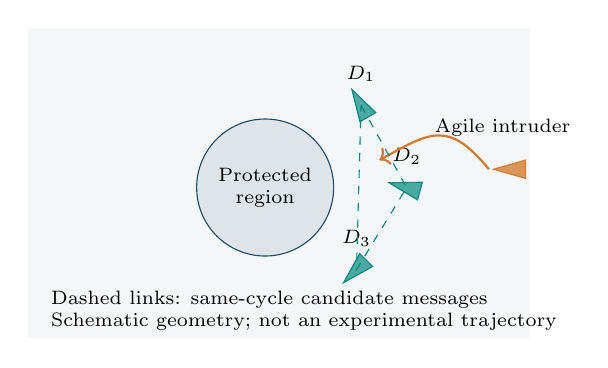
\begin{tikzpicture}[scale=.058,font=\scriptsize]
\fill[navy!5] (-52,-33) rectangle (58,35);
\draw[navy,fill=navy!15] (0,0) circle (15);
\node[align=center] at (0,0) {Protected\\region};
\foreach \x/\y/\a/\name in {21/18/120/1,31/0/165/2,20/-18/225/3}{
\begin{scope}[shift={(\x,\y)},rotate=\a]
\draw[fill=teal!70,draw=teal] (4,0)--(-3,2)--(-3,-2)--cycle;
\end{scope}
\node[above] at (\x,\y+3) {$D_{\name}$};}
\draw[fill=orange!80,draw=orange] (50,4)--(57,6)--(57,2)--cycle;
\node[above] at (52,9) {Agile intruder};
\draw[->,orange,thick] (49,4) .. controls (40,15) and (36,12) .. (25,6);
\draw[dashed,teal] (21,18)--(31,0)--(20,-18)--cycle;
\node[align=left,anchor=west] at (-49,-27) {Dashed links: same-cycle candidate messages\\Schematic geometry; not an experimental trajectory};
\end{tikzpicture}
\caption{Cooperative control composition for target defense. Dashed links carry concurrent candidate-control information; the drawing assigns no fixed maneuver roles. Defense succeeds through capture or survival to the 60-s deadline, with region entry and defender collision recorded separately.}
\label{fig:task}
\end{figure}

\section{Task and Control Model}
\subsection{Dynamics, observations, and outcomes}
Let $N$ homogeneous defenders protect a circular target region of radius $15$ m against one intruder. The numerical environment follows the released three-degree-of-freedom WAM-V model~\cite{tao},
\begin{equation}
 \dot\eta_i=R(\psi_i)\nu_i,\qquad
 M\dot\nu_i+C(\nu_i)\nu_i+D(\nu_i)\nu_i=\tau_i,
\end{equation}
with the source current perturbations and a $0.05$-s integration step. A command is held for four integration steps, giving a $0.2$-s control period. Differential thrust lies in $[-500,1000]$ N per thruster; intruder agility scales its thrust bounds. Observations contain target-relative and intruder-relative geometry, measured intruder velocity, Boids features, and teammate distance--bearing pairs. Candidate messages add measured defender position, heading, translational velocity, yaw rate, and both current action candidates. No future disturbance, true intruder agility, or centralized training state is an actor input.

We use \texttt{paper-parameters-v1}: a run terminates at actual target entry ($d_{AT}\leq15$ m), a defender separation at or below $5$ m, capture ($\min_i d_{iA}<5$ m), or $60$ s. This is also the priority order for simultaneous terminal events. Independent physical collision and breach flags are retained alongside that exclusive outcome. The deadline is an absorbing task termination, with zero bootstrap value.

\subsection{Control sources and nominal composition}
For the learning realization, Boids supplies pursuit, separation, alignment, and cohesion forces using the released parameters. A shared learned candidate $\ell_i\in(-1,1)^2$ maps to physical thrust $u_i^L=750\ell_i+250$. The mixed nominal control is
\begin{equation}
 u_i^{\rm nom}=\theta_i u_i^L+(1-\theta_i)u_i^B,\qquad 0\leq\theta_i\leq1.
 \label{eq:mix}
\end{equation}
We define \emph{control composition} as the state-dependent combination of control sources in the nominal command. The predictive realization in Section~\ref{sec:predictive-method} uses an interception prior and pursuit feedback; the learning realization uses the sources in~\eqref{eq:mix}. The candidate controls and team composition configuration are
\begin{equation}
 \mathcal A=\bigl((u_i^L,u_i^B)\bigr)_{i=1}^{N},\qquad
 \boldsymbol\Theta=(\theta_1,\ldots,\theta_N).
 \label{eq:configuration}
\end{equation}
Cooperative control composition seeks to match these local choices to inter-vessel interactions and the team task. Each blending coefficient describes the relative contribution of two sources to one nominal command: $\theta_i+(1-\theta_i)=1$. There is no shared cross-vessel coefficient budget or constraint $\sum_i\theta_i=1$. Local control authority is an interpretation of this relative contribution, not a transfer of actuator permissions.

For fixed candidate controls,
\begin{equation}
 \frac{\partial u_i^{\rm nom}}{\partial\theta_i}=u_i^L-u_i^B.
 \label{eq:composition-sensitivity}
\end{equation}
Thus coefficient variation translates into command variation through candidate disagreement. Every primary learning method then uses the same existing second-order CBF filter, with a $7$-m barrier separation, the released relaxed quadratic-program settings, and identical physical saturation. Writing $\mathbf u$ for the stacked thrust commands, execution is
\begin{equation}
 \mathbf u^{\rm exec}=\mathcal F_{\rm CBF}(s,\mathbf u^{\rm nom}).
 \label{eq:execution}
\end{equation}
The blending coefficient therefore characterizes nominal composition, not the final motion's proportional contribution from each source. Pursuit, lateral interception, and region maintenance are functions to identify in recorded trajectories. They are not roles assigned by large or small coefficients: Boids itself includes pursuit, and the learned branch receives task, formation, and collision feedback. Relaxed CBF feasibility is evaluated through measured collision outcomes.

\subsection{Task reward}
The defender reward retains the paper's task, formation, and collision terms. Target entry yields $-100$ to each defender; capture yields $100$ to a defender within the capture radius, $50$ within three capture radii, and zero task reward otherwise. Each colliding defender receives one $-50$ penalty. Writing $e_i=(p_A-p_i)/\|p_A-p_i\|$, $q=\sum_i e_i$, and $e_T=p_A/\|p_A\|$, the formation term is
\begin{equation}
 r_i^{\rm form}=\tfrac12 e_T^\top q/\max(\|q\|,\epsilon)-\|q\|/N.
\end{equation}
Terms are evaluated on terminal transitions too, with the exact released boundary comparisons retained in code. The joint learner uses $\bar r=N^{-1}\sum_i r_i$. Return, defense success, and capture time are distinct quantities throughout the evaluation.

\section{Learning Cooperative Control Composition}
The primary research object remains the original learned--Boids fusion. The two mechanisms below are implemented but have not yet established stable incremental task gains. A failed training run alone does not diagnose an action-space limitation.

\subsection{Candidate-control interaction-conditioned blending}
The first stage independently generates learned candidates from the shared ARBoids observation encoder. Its task and Boids encoders and masked mean teammate embedding feed the retained 512-unit decision backbone. Reparameterized Gaussian samples are squashed by $\tanh$ to form $\ell_i$. The second stage exchanges candidates from the same control instant. For each directed pair, a shared two-layer, 128-unit encoder receives
\begin{equation}
  z_{ij}=(\delta p_{ij}^{i}/60,\sin\delta\psi_{ij},\cos\delta\psi_{ij},
  \delta v_{ij}^{i}/5,\delta r_{ij},\ell_i,b_i,\ell_j,b_j),
 \label{eq:candidate-relations}
\end{equation}
where $b_i=(u_i^B-250)/750$ and superscript $i$ denotes rotation into defender $i$'s heading frame. For valid non-self neighbors $\mathcal N_i$, the candidate-interaction message and conditional blending policy are
\begin{equation}
 h_i^{\rm rel}=\frac{1}{|\mathcal N_i|}\sum_{j\in\mathcal N_i}f_\kappa(z_{ij}),\qquad
 \theta_i\sim\pi_\phi^g(\cdot\mid h_i,\ell_i,b_i,h_i^{\rm rel}).
 \label{eq:composition-policy}
\end{equation}
An empty neighbor mask yields a zero message. This representation conditions composition on current candidate relations; it imposes no requirement that different defenders use different coefficients. The gate mean adds a message-dependent residual to the original adapter logit; the residual initializes at zero. A learned gate log standard deviation initializes at $\log(0.1)$.

With $h_i$ the backbone feature and $\epsilon_i^g\sim\mathcal N(0,1)$,
\begin{equation}
 z_i^g=\mu_i^g(h_i,h_i^{\rm rel},\ell_i,b_i)+\sigma_i^g(h_i,h_i^{\rm rel})\epsilon_i^g,
 \quad \theta_i=\frac{\tanh z_i^g+1}{2}.
\end{equation}
Thus the joint density factorizes into a proposal stage and a conditional gate stage,
\begin{equation}
  \Pi_\phi(\ell,\boldsymbol\Theta\mid o)=\prod_i\pi_\phi^L(\ell_i\mid o_i)
 \prod_i\pi_\phi^g(\theta_i\mid h_i,h_i^{\rm rel},\ell_i,b_i).
\end{equation}
The gate log density includes both transformations:
\begin{equation}
 \log\pi_i^g=\log\mathcal N(z_i^g;\mu_i^g,\sigma_i^g)
 -\log(1-\tanh^2 z_i^g)+\log2.
\end{equation}
We evaluate the log-Jacobian in a stable softplus form. Gate losses backpropagate through the candidate messages when the proposal branch is unfrozen. Deterministic evaluation uses the transformed Gaussian means in both stages.

\begin{figure*}[t]
\centering
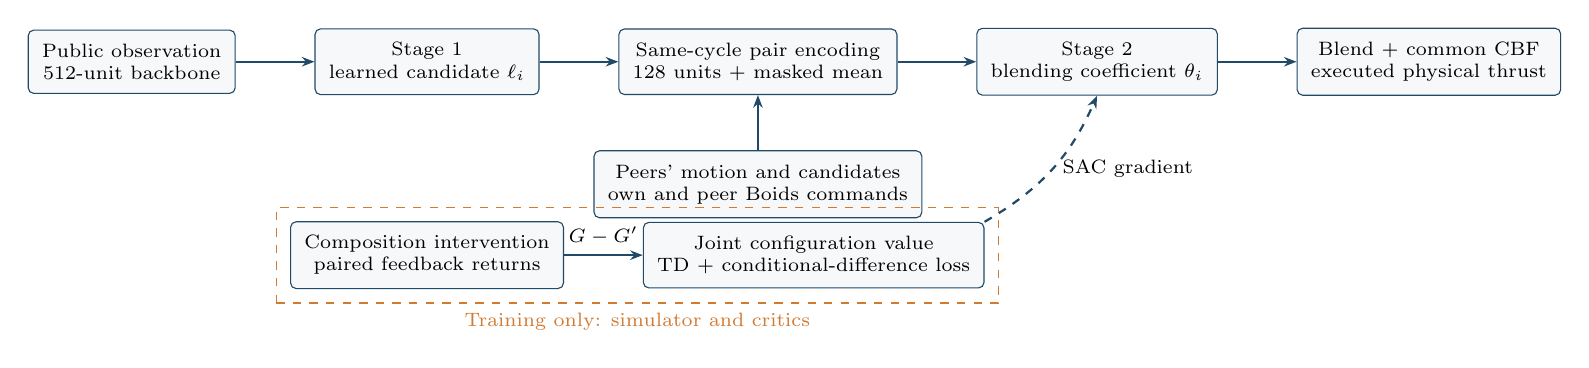
\begin{tikzpicture}[node distance=7mm and 10mm]
\node[box] (obs) {Public observation\\512-unit backbone};
\node[box,right=of obs] (cand) {Stage 1\\learned candidate $\ell_i$};
\node[box,right=of cand] (rel) {Same-cycle pair encoding\\128 units + masked mean};
\node[box,right=of rel] (gate) {Stage 2\\blending coefficient $\theta_i$};
\node[box,right=of gate] (cbf) {Blend + common CBF\\executed physical thrust};
\draw[flow] (obs)--(cand);\draw[flow] (cand)--(rel);\draw[flow] (rel)--(gate);\draw[flow] (gate)--(cbf);
\node[box,below=of rel] (peer) {Peers' motion and candidates\\own and peer Boids commands};
\draw[flow] (peer)--(rel);
\node[box,below=16mm of cand] (roll) {Composition intervention\\paired feedback returns};
\node[box,right=of roll] (critic) {Joint configuration value\\TD + conditional-difference loss};
\draw[flow] (roll)--node[above,font=\scriptsize] {$G-G'$}(critic);
\draw[flow,dashed] (critic.north east) to[bend right=18] node[right,font=\scriptsize] {SAC gradient} (gate.south);
\node[draw=orange,dashed,fit=(roll)(critic),inner sep=5pt,label={[font=\scriptsize,text=orange]below:Training only: simulator and critics}] {};
\end{tikzpicture}
\caption{The coupled policy and learning mechanism. Candidate-control relations condition local blending; paired composition interventions supervise conditional differences in the joint configuration value. Actor--critic updates connect that evaluation to the policy. Deployment uses the actor and common CBF.}
\label{fig:architecture}
\end{figure*}

\subsection{Joint configuration value and real-transition learning}
For policy $\Pi$, let $\mathcal Q^\Pi(s,\mathcal A,\boldsymbol\Theta)$ denote the team's soft value conditioned on the current state, candidate controls, and complete composition configuration. Holding $\mathcal A$ fixed distinguishes a change in composition from an arbitrary replacement of the candidate controls. A local value can also be defined by averaging over teammates' coefficients under their policy. Retaining the full configuration enables the critic to represent differences across those teammate choices instead of only their average. This is value-level configuration interaction, distinct from the candidate-interaction message in~\eqref{eq:composition-policy}.

In the implementation, $u_i^L$ is determined by $\ell_i$ and the Boids command by $s$, so the same value is represented as $Q^\Pi(s,a)$ with $a=(\ell,\boldsymbol\Theta)$. The transition includes the common CBF filter and subsequent vessel dynamics.

Each of two critics encodes a node containing a defender's centralized kinematic state, normalized composed nominal thrust, left--right thrust difference, and Boids candidate. The action coordinates are $v_i=\theta_i\ell_i+(1-\theta_i)b_i$, where the corresponding physical thrust is $750v_i+250$ N and $b_i$ is the normalized Boids candidate. Equivalent proposal--gate factorizations therefore receive exactly the same value, as they produce the same input to the CBF; the current action's entropy is outside $Q$. The audited state representation additionally includes the measured ground velocity used by the CBF and the vessel's normalized position in the simulator's obstacle traversal order. Relative-to-water velocity alone does not determine the CBF input, and the released APF opponent is order dependent. These four additional node scalars correct the conditioned state without changing either controller. A symmetric pair encoder takes the sum and absolute difference of node embeddings and pair distance. Masked means pool nodes and non-self pairs. The critic head receives both pools, the intruder state, agility, remaining task time, and $N/7$, and outputs one team value. Shared encoders accept two through seven defenders, but invariance to changes in the simulator's traversal order is not imposed. Centralized information is restricted to critic training. This corrected representation is versioned as \texttt{execution-v2}; historical checkpoints retain their original \texttt{dynamics-v1} interpretation and cannot silently resume under the new representation.

One replay record represents one complete team control cycle: observations, public kinematics, centralized state, proposals, all blending coefficients, actual filtered thrust, individual and mean rewards, next observations and states, and the terminal flag. Critic actions are $(\ell,\boldsymbol\Theta)$; filtered thrust is recorded for audit.

The entropy term uses the same per-defender scale as the mean team reward. For stage $z$, define
\begin{equation}
 e_\phi(o,a;z)=\frac{\ind[z=\mathrm{joint}]}{N}\sum_{i=1}^N
 \log\pi_\phi^L(\ell_i\mid o_i).
\end{equation}
During gate learning, the frozen proposal distribution supplies exogenous candidates and the gate optimizes physical task return. Joint learning regularizes the trainable proposal distribution at the per-defender scale. Gate sampling supports exploration, while its mean and variance learn through task value without a gate-density reward. For $a=(\ell,\boldsymbol\Theta)$, our real-data evaluator and soft actor--critic~\cite{sac} policy updates use
\begin{align}
 y&=\bar r+\gamma(1-d)\left[\tfrac12\sum_{k=1,2}\bar B_k(s',a')-\alpha e_\phi(o',a';z)\right],\\
 L_B&=\sum_k\E[(B_k(s,a)-\sg(y))^2],\\
 L_{\rm TD}&=\sum_k\E[(Q_k(s,a)-\sg(y))^2],\\
 L_\pi&=\E[\alpha e_\phi(o,a;z)-\min_kQ_k(s,a)].
\end{align}
The real-data evaluator averages its two heads for bootstrapping; policy improvement retains the main-critic minimum. Full, Same-info, No-candidate-interaction, Short, and Model-return share this choice. Truncated rollout tails use the same evaluator average, while the registered conditional-value diagnostics retain their original definition.
We use $\gamma=0.99$, target smoothing $0.005$, and minibatches of 4096 joint transitions. Adam learning rates are $10^{-4}$ for critics and $10^{-5}$ for the actor and temperature. Proposal temperature starts at $0.2$ and adapts during joint learning to a per-defender entropy target of $-2$; the gate stage has zero entropy cost and no temperature update. Each matched joint-learning arm has a main twin critic $Q$ and an independent twin bootstrap evaluator $B$, both with the same 512/128 widths and initialization. After initialization from complete real-episode returns, the evaluator receives only $L_B$ on real transitions, and its lagged copy follows $\bar B\leftarrow(1-\tau)\bar B+\tau B$. The main critic receives the real-transition loss and the arm's prescribed auxiliary loss. Auxiliary gradients and main-critic parameters never update $B$ or $\bar B$. Same-info retains the same evaluator updates; without auxiliary supervision its main and bootstrap critics remain identical. The additional evaluator updates are counted separately.

\subsection{Local composition intervention and conditional return difference}
Let $\boldsymbol\Theta^{(i)}=(\vartheta_i,\boldsymbol\Theta_{-i})$ mean replacing component $i$ by a reference coefficient $\vartheta_i$ while retaining the original indexing. The conditional value difference of this local composition change is
\begin{equation}
 \begin{aligned}
 \Delta_i^\Pi(s,\mathcal A,\boldsymbol\Theta;\vartheta_i)
 &=\mathcal Q^\Pi(s,\mathcal A,\boldsymbol\Theta)\\
 &\quad-\mathcal Q^\Pi(s,\mathcal A,\boldsymbol\Theta^{(i)}).
 \end{aligned}
 \label{eq:conditional-composition-value}
\end{equation}
For a captured training state, sample one common first joint action and a defender index $i$. Draw $\vartheta_i$ uniformly from $\{0,0.5,1\}$. The alternate first action $a^{(i)}$ fixes $s$, $\mathcal A$, and $\boldsymbol\Theta_{-i}$ and changes only $\theta_i$. Both branches start from separate complete copies of the same simulator state and share the same external random-number stream and policy sampling noise. From the second control cycle onward, every defender recomputes both policy stages using its own branch's evolved observations under the same frozen policy. The intervention is applied once; it does not fix the subsequent coefficients. The CBF, task reward, discount, and termination rules are identical in both branches.

For label batch $b$, freeze copies $(\Pi_b,\alpha_b,\bar B_b)$ of the policy, temperature, and tail evaluator. Let $H$ be the rollout horizon and $K\leq H$ the executed number of steps. Define
\begin{align}
 G_H(s,a)&=\sum_{k=0}^{K-1}\gamma^k\bar r_k
 -\alpha_b\sum_{k=1}^{K-1}\gamma^k e_{\phi_b}(o_k,a_k;z)\nonumber\\
 &\quad+\ind[\text{not terminal at }K]\gamma^K\bar V(s_K),\\
 \bar V(s_K)&=\tfrac12\sum_{j=1,2}\bar B_{b,j}(s_K,a_K)-\alpha_b e_{\phi_b}(o_K,a_K;z).
\end{align}
The prescribed first action has no entropy contribution, consistent with the soft $Q$ convention. The subsequent action sample used for a truncated tail is shared by noise across branches. The actor, temperature, and real-data tail evaluator are frozen for an entire label batch, and the resulting targets stop gradients. Full, No-candidate-interaction, and Model-return use $H=300$ and reach task termination, so their labels contain no learned tail; Short uses $H=10$ and the truncated expression above. The sampled training target is
\begin{equation}
 \widehat{\Delta G}_{H,i}=\frac{1}{R}\sum_{r=1}^{R}\bigl[G_H^{(r)}(s,a)-G_H^{(r)}(s,a^{(i)})\bigr].
 \label{eq:paired-composition-target}
\end{equation}
For training, $R=8$: the state, first action, and intervention remain fixed across repetitions; future environment and policy noise are independent across repetitions and shared within each pair. The label combines closed-loop simulated rewards with a frozen value tail when the horizon is truncated. Its within-state Monte Carlo standard error is recorded. Thus the supervision contains simulated consequences of the composition change, rather than only a difference between the current critic's own predictions. The ordinary-return control uses the mean of each branch over the same eight repetitions.

\begin{figure}[t]
\centering
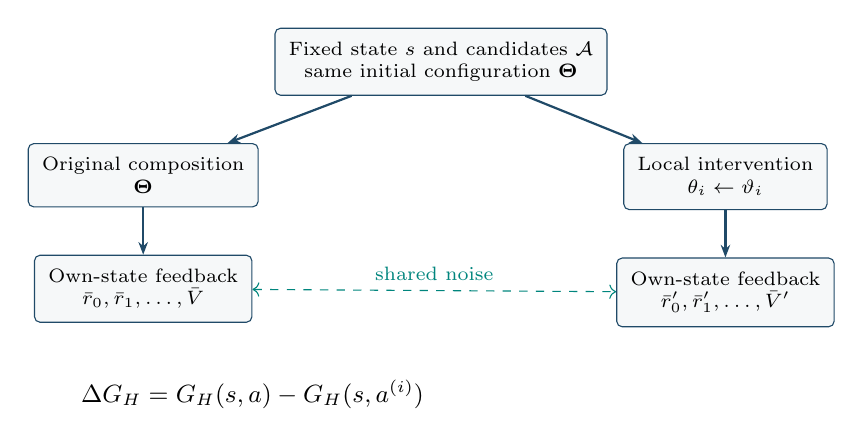
\begin{tikzpicture}[node distance=6mm and 2mm]
\node[box] (s) {Fixed state $s$ and candidates $\mathcal A$\\same initial configuration $\boldsymbol\Theta$};
\node[box,below left=of s] (a) {Original composition\\$\boldsymbol\Theta$};
\node[box,below right=of s] (b) {Local intervention\\$\theta_i\leftarrow\vartheta_i$};
\node[box,below=of a] (fa) {Own-state feedback\\$\bar r_0,\bar r_1,\ldots,\bar V$};
\node[box,below=of b] (fb) {Own-state feedback\\$\bar r'_0,\bar r'_1,\ldots,\bar V'$};
\draw[flow] (s)--(a);\draw[flow] (s)--(b);\draw[flow] (a)--(fa);\draw[flow] (b)--(fb);
\draw[<->,dashed,teal] (fa)--node[above,font=\scriptsize] {shared noise}(fb);
\node[below=6mm of fa.south east,anchor=north,font=\small] {$\Delta G_H=G_H(s,a)-G_H(s,a^{(i)})$};
\end{tikzpicture}
\caption{A local composition intervention fixes the current state, both candidate controls of every defender, and all other current coefficients. Later actions follow the same policy on each branch's own state. The label estimates a conditional soft-return difference for the composition variable.}
\label{fig:intervention}
\end{figure}

\subsection{Composition-specific conditional value supervision}
The complete method adds
\begin{equation}
 L_\Delta=\sum_{j=1}^2\E\left[\left(Q_j(s,a)-Q_j(s,a^{(i)})-
  \sg\{\widehat{\Delta G}_{H,i}\}\right)^2\right]
\end{equation}
to the real-transition loss: $L_Q=L_{\rm TD}+0.1L_\Delta$. The ordinary model-return control uses
\begin{equation}
 \begin{aligned}
  L_G=\tfrac12\sum_j\E\bigl[&(Q_j(s,a)-\sg G_H(s,a))^2\\
  &+(Q_j(s,a^{(i)})-\sg G_H(s,a^{(i)}))^2\bigr].
 \end{aligned}
\end{equation}
Both objectives consume both branches. Each method generates labels under its own current frozen policy. The random-seed rule, snapshot sampling, intervention distribution, pair count, and horizon are matched; trajectories need not coincide after policies diverge. This avoids assigning another policy's continuation return to a method's own conditional value. Real transitions learn task value, paired consequences distinguish the conditional effect of local composition, and the actor objective transmits that evaluation to the blending policy. This supervision targets the composition variable and its closed-loop consequences within actor--critic learning; it does not introduce a separate role or responsibility allocator.

The long variants run to actual task termination, for at most $H=300$ control cycles (the remaining portion of the 60-s episode); the short variant uses $H=10$ (2 s). After critic warmup, every 1000 real transitions produces 64 fixed root interventions drawn from a rolling pool of 256 snapshots sampled every 16 transitions. Each root uses eight paired futures. The 64 averaged labels are reused between refreshes alongside the 4096-transition real minibatch, a ratio of $1/64$; rollout generation does not cover all 4096 samples at every update. A new batch replaces the previous labels. The exact conditional-return interpretation refers to the generating snapshot $\Pi_b$; reusing labels while the actor changes introduces a policy-lag approximation. Fixed-policy critic diagnostics hold this continuation policy constant. No auxiliary rollout transition enters the ordinary replay. The implementation uses the complete training simulator for labels. Long-label error includes finite-sample variability; Short additionally depends on a bootstrapped tail. Real transitions, simulated transitions, gradient updates, and wall time are counted separately.

\subsection{Focused diagnostic sequence}
The opportunity experiment freezes the original pretrained policy and tests finite, single-vessel blending interventions. It records nominal and post-CBF command changes and complete real-environment outcomes. Four search futures select a candidate; eight disjoint future realizations then evaluate the selected candidate against the unmodified action. This separation distinguishes an executable, repeatable opportunity from choosing an intervention that happened to benefit one disturbance sequence.

Two selection rules are compared on the same branches. One minimizes capped capture time while preserving the search sample's observed capture, breach, and collision outcomes. The other maximizes the original discounted paper reward with $\gamma=0.99$. Their independent-future outcomes examine whether improvement of the training objective agrees with improvement of the task. This deterministic-policy diagnostic has no entropy term and must not be used as a value target for a different stochastic continuation policy.

Only if useful fusion opportunities are supported will matched information comparisons examine candidate-relation encoding against state-only neighbor encoding. These comparisons retain corresponding state information, comparable parameter counts, and identical training data and budgets. Conditional-value tests then compare real TD, matched absolute-return supervision, and return-difference supervision on independently sampled interventions under the same frozen continuation policy. Finally, actor-gradient direction and closed-loop task changes test whether value improvements are usable by the adapter. Larger training budgets and a hierarchical composition upgrade are decisions to be made from these results.

\section{Independent Predictive Control Reference}
\label{sec:predictive-method}
\subsection{Interception prior and pointwise residual}
The interception goals are $g_j=p_A+\ell_j e_\perp$, where $e_\perp$ is perpendicular to the target--intruder radial direction and $N$ offsets $\ell_j$ are equally spaced over $[-28,28]$~m. Minimum-cost assignment uses $c_{ij}=\|g_j-p_i\|/3.2+0.6|\varepsilon_{ij}|$, with wrapped heading error $\varepsilon_{ij}$. For either an assigned goal or direct pursuit of the current intruder position, let $d_i$ and $\varepsilon_i$ denote goal distance and heading error, $v_i$ measured forward speed, and $r_i$ yaw rate. The common feedback law is
\begin{align}
 v_i^*&=3.2\min(d_i/5,1)\max(\cos\varepsilon_i,0),\\
 F_i&=\tfrac12\bigl(100v_i^*+150(v_i^*)^2+400(v_i^*-v_i)\bigr),\\
 Y_i&=900\varepsilon_i-700r_i,\\
 u_i(g)&=\operatorname{clip}([F_i+Y_i,F_i-Y_i],-500,1000).
\end{align}
All compositions use these same candidate laws and the common execution filter.

The predictive realization preserves a strong cooperative interception prior and selects residual capture maneuvers by their joint feedback consequences. Let $u_i^0(s)$ denote the command from a minimum-cost assignment to lateral interception goals and $u_i^p(s)$ a direct-pursuit command. The residual composition is
\begin{equation}
 \begin{aligned}
 u_i(s;m)&=u_i^0(s)+m_i\bigl(u_i^p(s)-u_i^0(s)\bigr),\\
 &m\in\{0,1\}^N,\quad \|m\|_0\leq2.
 \end{aligned}
 \label{eq:structured-residual}
\end{equation}
The assignment is a control prior: assignment-based capture-time optimization already has a substantial precedent~\cite{zhang-assignment}, as does combining feedback control with learned residuals~\cite{johannink}. Here the evaluated mechanism is the joint, sustained consequence of choosing which defenders depart from that prior. Six defenders give 22 compositions. Every 2~s, each composition is simulated with feedback for the 2-s commitment and a 20-s continuation under the same composition. The predictor ranks collision, breach, and estimated capture time lexicographically; nonzero residuals incur a fixed 0.15-s departure cost. Physical commands and the common CBF are recomputed every 0.2~s. The zero composition retains the prior exactly. Attacker agility is inferred causally from past measurements on the common range $[1,8]$; the controller does not receive true agility or future disturbances.

The matched additive control uses the same candidates and computes the same 22 forecasts, but selects with
\begin{equation}
 \widetilde C(s,m)=C(s,0)+\sum_i m_i\bigl[C(s,\mathbf e^{(i)})-C(s,0)\bigr],
\end{equation}
where $\mathbf e^{(i)}$ is a singleton pursuit composition and $C$ scalarizes predicted collision, breach, and time using weights 360, 180, and 1. This control removes joint-composition consequences from selection while preserving forecast budget. A short control retains joint selection but removes the 20-s continuation. The existing long predictor uses the same expanded agility-observer range; its original upper bound of 3.25 would be inappropriate for these conditions.

\subsection{Conditional teammate response}
Conditioning the remaining defenders' control roles on the selected capture maneuvers strengthens both task performance and the measured interaction effect. A pointwise pursuit residual leaves non-pursuing defenders in roles assigned under the assumption that the whole team is guarding. We instead complete the guard assignment after choosing the pursuing set $P(m)=\{i:m_i=1\}$. Capture roles replace the $|P(m)|$ innermost lateral interception roles; remaining defenders are assigned to the remaining roles by minimum total arrival cost. Symmetric central-role ties are resolved by the smaller total assignment cost. Assignment itself is an established control prior~\cite{zhang-assignment}; the tested change is its conditioning on the residual composition and the joint evaluation of the resulting feedback.

Let $g^*(s,m)$ denote that assignment and $u_{i,g^*}(s)$ the corresponding guard command. The coordinated residual is
\begin{equation}
 \begin{aligned}
 u_i^G(s,m)&=\begin{cases}
 u_i^p(s),&m_i=1,\\
 u_{i,g^*(s,m)}(s),&m_i=0,
 \end{cases}\\
 \delta u_i(s,m)&=u_i^G(s,m)-u_i^0(s).
 \end{aligned}
\end{equation}
The zero composition exactly recovers the original joint interception prior. A one-bit composition change includes its induced teammate guard responses, so its value concerns a coordinated composition intervention. The same 22 binary compositions, 2-s commitment, 20-s predictive continuation, public observations, agility observer, and 0.2-s physical feedback are retained. Guard assignments are recomputed from the current state during both forecasts and execution. The matched additive comparator uses these same completed controls and all 22 forecasts, replacing joint-composition selection by the sum of single-defender cost changes defined above.

\subsection{Adaptive response selection}
To adapt the composition to the current state, we select the teammate response together with the pursuing set. Let $\rho\in\{0,1\}$ indicate whether the remaining defenders reassign their guard roles. The resulting composition is
\begin{equation}
 \begin{aligned}
 u_i(s;m,\rho)={}&u_i^0+m_i(u_i^p-u_i^0)\\
 &+\rho(1-m_i)\bigl(u_i^G(s,m)-u_i^0\bigr).
 \end{aligned}
 \label{eq:adaptive-guard}
\end{equation}
The shared zero composition and 21 nonzero pursuit compositions in each response mode give 43 candidates. We identify $a_i^C(s,z)=u_i(s;m,\rho)$. The high-level student and teacher share this operator. Teacher prediction selects $(m,\rho)$ under the same horizon and physical feedback. The matched additive control evaluates the same 43 candidates, reconstructs costs from single-defender differences within each response mode, and then selects across both modes. The matched short control also retains all 43 candidates.

\section{Experimental Design and Results}
%% BEGIN GENERATED RESULTS
\subsection{Current original-mechanism investigation}
The following critic experiments used the pre-audit state representation. A subsequent consistency audit identified missing CBF velocity information and an invalid permutation assumption for the order-dependent APF opponent. Their corrections pass analytic, finite-difference, and execution regression checks; task-level gains from the corrected representation have not yet been evaluated. Thus the historical results diagnose those checkpoints and do not establish that the two original mechanisms are intrinsically ineffective.
The original learned--Boids opportunity test used 48 independent source-policy states: 16 each with three and six defenders at agility 2.25, and eight each with six defenders at agility 4 and 6. All 48 admit a legal single-vessel blending change that alters actual post-CBF thrust. Each candidate changes only the current focal coefficient; subsequent controls resume the same frozen source policy on each branch's own state. Four shared search futures selected a candidate, followed by eight new paired futures. Task-selected capped-time differences were $-0.497$, $-1.427$, $-0.919$, and $-2.084$~s in the four conditions, respectively; every condition's exploratory state-bootstrap interval includes zero. The descriptive equal-state average is $-1.142$~s, with a post-hoc stratified 95\% interval of $[-2.418,0.072]$~s. The within-state standard deviation of a single paired time difference is 12.521~s. Reward-selected interventions give a similar uncertain mean change, $-1.228$~s. These outcomes establish executable action variation, but neither stable improvement nor impossibility of improvement.

A separate frozen-critic direction probe evaluates the v8 Full 10k checkpoint without an actor update. At each state, it chooses the vessel with largest absolute derivative of $\min(Q_1,Q_2)$ with respect to its coefficient and tests a clipped 0.1 change in that direction. An initial source-state probe includes six-vessel conditions, outside this critic's three-vessel training distribution; those cases are only extrapolation diagnostics. The subsequent check uses one uniformly sampled pre-action state from each of 64 new complete episodes of the checkpoint's own stochastic policy, under its three-vessel, agility-$2.25\pm0.5$ training conditions. Sixteen paired complete futures per action use the same frozen continuation policy and training return convention. Predicted mean improvement is 0.163, versus measured improvement 0.039 (95\% interval $[-0.327,0.424]$). The corresponding capped-time difference is $-0.004$~s ($[-0.284,0.274]$). Conditional-value MAE is 0.670, versus 0.608 for a zero-difference predictor.

In 35 of these 64 states, the proposed increase changes joint executed thrust by less than 1~N; no nominal change greater than 1~N is reduced below that threshold by the CBF. Coefficients near zero or one account for 32.8\% and 91.7\% of the 192 vessel-level outputs of the 5k and 10k checkpoints on these same states. Thus the observed failure includes severe gate drift and many almost ineffective outward changes. This coordinate probe is not a shared-parameter actor update and does not isolate the cause of that drift.

The subsequent matched critic experiment freezes the original deterministic policy. Three defenders face agility $2.25\pm0.5$; 256 training episodes provide 24195 real transitions, and 128 other episodes supply independent test roots. One uniformly sampled pre-action state per episode is evaluated with its current action and three single-vessel alternatives, $\theta_i\in\{0,0.5,1\}$, over eight complete paired futures. All arms share the same 512/128 twin-critic architecture, real minibatches, TD-only lagged targets, and model-return samples. A common 1500-update state-value warmup precedes 3000 fixed-policy critic updates. Auxiliary weight is 0.1. Initializations 42 and 101 share the dataset and are not independent data replications. No actor is updated or test-based checkpoint selected.
\begin{table}[t]
\caption{Fixed-policy critic diagnostic on 128 independent states. Time changes follow one selected intervention and then the frozen source policy.}
\label{tab:fixed-critic}\centering\small
\begin{tabular}{@{}llrr@{}}\toprule
Seed & Supervision & $\Delta Q$ MAE & $\Delta T_{60}$ (s)\\\midrule
42 & TD & 2.505 & +0.111\\
42 & TD + absolute & 2.469 & +0.217\\
42 & TD + difference & 2.483 & +0.134\\
101 & TD & 2.499 & +0.134\\
101 & TD + absolute & 2.429 & +0.206\\
101 & TD + difference & 2.459 & +0.080\\
--- & Zero difference & 2.088 & ---\\\bottomrule
\end{tabular}
\end{table}
All learned difference errors exceed the zero predictor (Table~\ref{tab:fixed-critic}), and all exploratory paired time intervals include zero. Difference supervision does not outperform matched absolute supervision. The estimated noise variance of an eight-future difference mean is 11.403, compared with an observed second moment of 12.847. These results identify difficult conditional-value generalization even without actor drift; they do not establish its unique cause. The experiment uses 681244 simulated steps. Critic-selected actions use centralized state and are diagnostic probes, not a deployed learned actor.

One targeted development test separates the TD baseline from the conditional response, $Q(s,a)=B_{\rm TD}(s,a_\pi)+A(s,a)-A(s,a_\pi)$. The same frozen TD baseline and network architecture are used for both absolute and difference fitting, with initially zero action-input weights and 3000 matched updates. On the now-reused development states, difference-supervised MAE worsens to 5.109 and 5.327; time changes are $+0.267$ and $+0.151$~s, with intervals including zero. Absolute-supervised MAE is 18.863 and 21.070. Reduced training loss therefore did not generalize. This correction is rejected and is not added to the main algorithm; no new complete SAC run follows these diagnostics. The incremental value of candidate-interaction information remains to be isolated.
%% END GENERATED RESULTS

\subsection{Adaptive joint composition: held-out task evidence}
The adaptive method and its four primary references were then frozen before 256 unused scenarios, again balanced between agility 4 and 6. Fixed completion was declared a secondary comparison for preservation of the preceding strong result, rather than another reference requiring a further 10\% speed gain. Table~\ref{tab:adaptive-guard} retains all six methods and all 1536 episodes.
\begin{table}[t]
\caption{Fresh adaptive-composition confirmation, 256 paired scenarios}
\label{tab:adaptive-guard}\centering\small
\begin{tabular}{@{}lrrr@{}}\toprule
Controller & Time (s) & Captures & Successes\\\midrule
Adaptive joint & 21.103 & 256 & 256\\
Adaptive additive & 26.417 & 251 & 255\\
Adaptive short & 30.245 & 244 & 253\\
Fixed initial roles & 31.028 & 244 & 256\\
Existing long predictor & 30.666 & 240 & 256\\
Fixed guard completion & 19.814 & 256 & 256\\\bottomrule
\end{tabular}
\end{table}
All six methods have zero collisions. Adaptive joint selection is 20.12\%, 30.23\%, 31.99\%, and 31.18\% faster than the four primary references. Accounting for the linked random streams in 128 blocks, the respective simultaneous 98.75\% paired time intervals are $[-7.458,-3.248]$, $[-11.323,-7.019]$, $[-12.373,-7.532]$, and $[-11.905,-7.240]$~s. The dependence-aware binary bound uses that a positive two-stratum block difference is at least $1/2$ and a negative one has magnitude at most one; two Clopper--Pearson tails of 0.025 bound the corresponding event probabilities. All capture and success lower bounds exceed $-3$ percentage points; the smallest success bound is $-2.841$ points. Both the original registered analysis and this additional analysis, specified before inspecting the new task outcomes, pass all four combined criteria. The secondary fixed-completion controller is 1.289~s faster on this bank with identical observed outcomes; an exploratory paired-block 95\% interval for adaptive-minus-fixed time is $[0.290,2.306]$~s. Thus the new bank establishes superiority over the primary references and retains a strong task result, but does not establish dominance over fixed completion.

\subsubsection{Replication with disjoint random streams}
The unchanged controller was frozen again before 256 further scenarios, with 128 in each agility stratum. Stratum seed ranges are now separated by $10^7$ and future disturbances retain their $10^6$ offset, making all initialization and disturbance streams disjoint within this bank and from the preceding bank. Frozen-source comparison confirms identical control logic; only the evaluation driver's seed allocation and validation changed. The replication declares adaptive additive selection and the existing long predictor as its two primary references, with fixed completion retained as a secondary reference.
\begin{table}[t]
\caption{Independent-stream replication, 256 paired scenarios}
\label{tab:adaptive-replication}\centering\small
\begin{tabular}{@{}lrrr@{}}\toprule
Controller & Time (s) & Captures & Successes\\\midrule
Adaptive joint & 20.523 & 256 & 256\\
Adaptive additive & 26.247 & 255 & 256\\
Existing long predictor & 32.113 & 238 & 256\\
Fixed guard completion & 20.205 & 256 & 256\\\bottomrule
\end{tabular}
\end{table}
All methods again have zero collisions. The joint-versus-additive time reduction repeats at 21.81\%, with a paired difference of $-5.723$~s and simultaneous 97.5\% interval $[-7.473,-3.986]$~s. Against the existing long predictor, the reduction is 36.09\%, with difference $-11.589$~s and interval $[-13.696,-9.496]$~s. All capture and success noninferiority checks pass; the success lower bound is $-1.431$ percentage points. Both primary combined gates pass. Adaptive joint times are 19.522 and 21.525~s at agility 4 and 6, compared with additive times of 23.545 and 28.948~s. Fixed completion is 0.318~s faster on average; its exploratory adaptive-minus-fixed 95\% paired interval is $[-0.640,1.292]$~s. The two untouched-controller banks together yield 512 captures, no breaches, and no collisions for adaptive joint selection, while preserving the separately reported primary analyses and the speed comparison with fixed completion.

\subsubsection{Computation and exact forecast pruning}
The expanded bank admits an exact elapsed-time bound. Once a completed forecast with no predicted collision or breach supplies a cost $B$, an unfinished forecast cannot win if its elapsed time plus departure cost is strictly greater than $B$: its eventual nonfailure estimate is no smaller, and predicted failure is worse lexicographically. The original candidate order resolves ties. On two complete development trajectories, bounded parallel evaluation preserves all 189 physical commands and selected forecast trajectories elementwise. With other experiments stopped, 19 warm planning calls have median 94.13~ms, p95 191.61~ms, and maximum 217.87~ms, compared with unbounded parallel p95 346.23~ms. One bounded call exceeds the 200-ms interval. Ordinary feedback has p95 3.04~ms; cold startup and first prediction take 8.59~s. This is measured computation performance, not a hard real-time guarantee. Independent task comparisons use all complete forecasts for each method.

\subsection{Conditional guard completion: strengthened interaction evidence}
\label{sec:guard-completion}
We evaluate the conditional teammate-response operator in Section~\ref{sec:predictive-method}.

Following development on 16 scenarios, the method and analysis were frozen before 128 unused six-defender scenarios, balanced between attacker thrust multipliers 4 and 6. Initial states, disturbances, CBF filtering, and the 60-s capped capture metric are paired. All scenarios are retained.
\begin{table}[t]
\caption{Independent conditional-guard evaluation, 128 paired scenarios}
\label{tab:guard-completion}\centering\small
\begin{tabular}{@{}lrr@{}}\toprule
Controller & Time (s) & Captures\\\midrule
Joint guard completion & 19.858 & 128\\
Original joint predictor & 24.888 & 126\\
Additive guard completion & 25.027 & 127\\\bottomrule
\end{tabular}
\end{table}
All three controllers achieve 128 defense successes and zero collisions. Joint guard completion reduces capped time by 20.21\% relative to the original strong joint predictor and 20.65\% relative to matched additive completion. The paired differences are $-5.030$ and $-5.169$~s, with simultaneous 97.5\% stratified bootstrap intervals $[-7.411,-2.762]$ and $[-7.405,-2.998]$~s, using 20000 draws. Both agility strata improve: the new controller takes 18.412 and 21.303~s, versus 23.772 and 26.003~s for the original predictor and 23.397 and 26.656~s for additive completion. Both contrasts pass the predeclared combined gate of at least 10\% mean time reduction, adjusted intervals below zero, and preserved task outcomes, including the one-sided 95\%, $-3$-percentage-point capture and success noninferiority checks. This result establishes task and interaction gains for conditional guard completion; the earlier pointwise method's failed tests below retain their original conclusions.

A second independently frozen bank contains 256 further scenarios, again balanced between the two agility strata. Joint completion takes 19.863~s, versus 24.823~s for matched additive completion, 29.913~s for matched short prediction, 30.257~s for fixed initial roles, and 32.370~s for the existing long predictor. The respective improvements are 19.98\%, 33.60\%, 34.35\%, and 38.64\%; simultaneous 98.75\% paired difference intervals are $[-6.845,-3.100]$, $[-12.545,-7.574]$, $[-12.683,-8.197]$, and $[-14.913,-10.071]$~s. Capture counts are 254, 254, 243, 246, and 230; defense successes are 254, 254, 255, 254, and 256, respectively. All methods have zero collisions. The time advantage and joint-versus-additive effect repeat, and all capture and success noninferiority checks pass. However, two target breaches make observed defense success lower than short and existing long prediction, so the full four-reference combined gate does not pass its additional observed-success requirement. The additive and fixed-role contrasts pass their complete criteria. These failures remain part of the reported evidence; diagnosing them does not convert the same scenarios into independent tests of a revised method.

As an inexpensive development challenge, directly assigning the nearest one or two defenders to pursue while completing the guard roles does not reproduce this benefit. With the same 2-s role commitment, their capped times are 33.150/32.825 and 28.750/44.125~s at agility 4/6, compared with 17.925/23.750~s for joint predictive completion on those 16 development scenarios. The stronger-agility rule controls also lose captures and defense successes. These small development comparisons motivated the independent test; they are kept separate from its inferential results.

Reusing composition-dependent role layouts and computing each state-dependent candidate set once removes redundant work without changing the control law. All 16800 candidate commands checked across 720 physical states with four, six, or eight defenders agree elementwise with the frozen implementation. On two complete six-defender development trajectories, serial and 22-worker parallel execution also agree in all 167 physical commands and selected plans. With other experiments stopped, the 16 warm planning calls have parallel p95 latency 156.36~ms and maximum 160.28~ms, versus serial p95 2950.37~ms, on the same 20-core CPU allocation reported below. All warm calls meet the 200-ms control interval; ordinary feedback has p95 2.93~ms. Pool startup and first prediction take 8.52~s. These measurements establish timing feasibility on the measured trajectories, with cold startup reported separately.

An audit of the random streams identifies dependence across agility strata: a scenario's disturbance seed equals its initialization seed plus $10^6$, which is also the next stratum's same-index initialization seed. An additional conservative analysis therefore resamples same-index strata together. It preserves both first-bank time effects, with 97.5\% intervals $[-7.117,-2.912]$ and $[-7.494,-2.925]$~s, and all four second-bank time intervals remain below zero. However, the first bank supplies only 64 independent stream blocks; its zero success difference has a conservative one-sided lower bound of $-5.60$ percentage points. In the second bank's 128 blocks, success lower bounds are approximately $-5.4$ to $-5.5$ percentage points. The original registered outputs above are retained, but their nominal noninferiority passes do not establish dependence-aware reliability within the prescribed three-point margin. The task-time and interaction benefits survive this audit; further confirmation uses disjoint initialization and disturbance seed ranges.

\subsubsection{Development of adaptive teammate response}
The two observed breaches motivate the adaptive response family in~\eqref{eq:adaptive-guard}.

On the reused 256-scenario bank, adaptive joint selection takes 20.178~s, with 255 captures, 256 defense successes, and zero collisions; matched adaptive additive selection takes 25.435~s, with 252 captures, 255 successes, and zero collisions. Relative to fixed completion, mean time increases by 0.316~s while both observed breaches are removed. A late-expansion variant, which exposes the second response mode only after every guard forecast predicts failure, does not repair either breach and is discarded. These findings are development evidence.

\subsection{Structured predictive compositions: completed task evidence}
\label{sec:structured-prediction}
The pointwise reference in~\eqref{eq:structured-residual} retains the original guard assignment.

Before evaluation, the implementation, comparisons, and analysis were frozen. The independent bank contains 128 six-defender scenarios at agility 4 and 128 at agility 6, paired across all five methods. Agility is an attacker thrust multiplier, not speed in metres per second. Initial states, disturbances, 60-s task outcomes, and safety filtering are common. All scenarios are retained, and a failure to capture is charged 60~s.
\begin{table}[t]
\caption{Frozen predictive-composition evaluation: capped time, 256 paired scenarios}
\label{tab:structured-prediction}\centering\small
\begin{tabular}{@{}lrrr@{}}\toprule
Controller & Time (s) & Captures & Successes\\\midrule
Joint interception prior & 31.146 & 244 & 253\\
Joint sustained prediction & 25.281 & 256 & 256\\
Additive composition selection & 27.331 & 250 & 255\\
Joint short prediction & 29.997 & 245 & 254\\
Existing long predictor & 31.312 & 237 & 256\\\bottomrule
\end{tabular}
\end{table}
Every method has zero observed collisions. Joint sustained prediction reduces mean capped time by 18.83\% relative to the interception prior, 15.72\% relative to short prediction, and 19.26\% relative to the existing long predictor. Their paired differences are $-5.865$, $-4.716$, and $-6.030$~s, with simultaneous 98.75\% bootstrap intervals $[-8.309,-3.414]$, $[-6.852,-2.550]$, and $[-8.672,-3.377]$~s, respectively. The analysis resamples scenarios within agility strata with 20000 draws and controls the four time comparisons at familywise level 0.05.

The additive contrast improves by 7.50\% ($-2.050$~s), but its adjusted interval is $[-4.106,0.032]$~s. Consequently the predeclared combined gate---at least 10\% time reduction against every reference, simultaneous intervals excluding zero, and preserved task outcomes---does not pass. All capture and success comparisons pass the separate one-sided 95\% noninferiority criterion of $-3$ percentage points, using conservative paired binomial bounds.

A separately frozen interaction replication uses another 256 scenarios with the same two agility strata and unchanged controllers. Joint and additive selection take 25.972 and 26.445~s, with 252 and 253 captures; both achieve 256 defense successes and zero collisions. Their difference is $-0.473$~s (95\% paired interval $[-2.263,1.363]$~s), and the conservative capture-difference lower bound is $-3.71$ percentage points. This replication does not pass its prespecified interaction-benefit and capture-preservation criteria. It does not replace the earlier failed combined gate. A supplementary fixed-assignment controller on these same new scenarios takes 30.639~s, with 243 captures, 254 defense successes, and zero collisions. Joint prediction is 15.23\% faster than this simple strong reference ($-4.667$~s; 95\% paired interval $[-6.753,-2.613]$~s), with capture and success noninferiority retained. For the pointwise residual in~\eqref{eq:structured-residual}, the task advantage over role assignment repeats, whereas its incremental joint-selection advantage over an additive predictor is not established.

These results belong to the structured online predictor. Learned conditional-value replacements tested on separate development scenes have not preserved its task advantage and do not establish a residual-RL benefit. A subsequent fitted-value pilot changes one composition coefficient for a 2-s block, then resumes the same frozen predictive policy in both branches. A 17-parameter correction fits the paired real-return difference relative to the model estimate; its matched control fits absolute returns from the same data. Each training state uses two independent paired futures. A development benefit of 0.85~s at correction strength 0.25 did not repeat: two independent training datasets evaluated on 128 shared new scenarios give conditional-versus-uncorrected and conditional-versus-absolute time differences of $+0.417$ and $+0.611$~s. Their crossed training-dataset/scenario bootstrap 97.5\% intervals are $[-1.445,2.167]$ and $[-1.052,2.384]$~s. The analysis rule was recorded after launch but before reading these evaluation outcomes. Both training replicates and all scenarios are retained; this learned correction is not adopted. Increasing to eight paired futures on exactly the same training states also fails to improve control: the two conditional corrections take 27.150 and 27.503~s on the shared 64-scenario development bank, versus 25.472~s uncorrected. These additional development outcomes do not support further replication-only training for this linear correction. The released APF opponent is sensitive to defender ordering, which is held fixed and identical across methods; broader opponent robustness remains to be established.

Candidate forecasts can be executed concurrently without changing the decision rule. After other experiment processes stopped, a 22-worker implementation was compared with serial execution on four complete development trajectories: six and eight defenders at agility 4 and 6, on an Intel Xeon Platinum 8470Q host with a 20-core allocation. All 389 executed commands, selected compositions, and selected forecast trajectories agree elementwise. Among the 22 warm six-defender planning calls, parallel p95 latency is 175.35~ms versus 2973.44~ms serially; the parallel maximum is 180.12~ms, below the 200-ms control interval. Its 194 ordinary feedback calls have p95 latency 2.87~ms. Eight-defender planning still has p95 latency 343.36~ms and 12 of 17 warm calls exceed 200~ms. Six-defender pool startup and first prediction take 8.73~s and are reported separately. This demonstrates preserved task behavior and timing feasibility on the measured six-defender trajectories, not a general deadline guarantee. No new VRX result is claimed.

\subsection{Alternative composition-student pilot}
A completed alternative pilot froze the 43-candidate pursuit--guard operator and learned only its composition choice, with continuous residuals set to zero. The structured student scored actual candidate-conditioned teammate responses; a flat 43-way student received the same public measurements and causal command history. Both used the same 256 teacher training episodes, 64 episode-separated validation episodes, soft behavior-cloning objective, 6000 updates, and training seeds 42 and 101. All 43 teacher score tuples were retained at each of 3504 labeled states. Initial and physical-future streams were disjoint across data partitions.

On 64 new paired test scenes at agility 4 and 6, both teachers captured every intruder without breaches or collisions. The structured students did not retain that performance (Table~\ref{tab:student-pilot}). Their validation preference losses were only slightly below the flat students', and the task advantage over the flat architecture was inconsistent across training seeds. All methods used the same CBF and had zero collisions.
\begin{table}[t]
\caption{Completed alternative student pilot, 64 new test scenes}
\label{tab:student-pilot}\centering\small
\begin{tabular}{@{}lrrr@{}}\toprule
Method & Time (s) & Captures & Breaches\\\midrule
43-candidate teacher & 22.044 & 64 & 0\\
22-candidate teacher & 20.353 & 64 & 0\\
Structured student, 42 & 31.438 & 61 & 2\\
Structured student, 101 & 33.669 & 59 & 2\\
Flat student, 42 & 34.494 & 58 & 4\\
Flat student, 101 & 33.713 & 55 & 2\\
Joint interception prior & 31.788 & 60 & 0\\
ARBoids+CBF & 40.916 & 46 & 8\\\bottomrule
\end{tabular}
\end{table}
Neither structured seed passed the declared development retention screen. This is evidence about this student and training protocol, not evidence that the original continuous fusion mechanism is invalid. The pilot remains an alternative-route record; no further architecture expansion is underway.



\subsection{Earlier evidence under its original protocol}
\label{sec:earlier}
Earlier online-selection experiments motivate both the research object and the learning signal. Under the same instantaneous risk objective, independent and joint coefficient selection achieved 403/512 and 433/512 successes, respectively, with collisions decreasing from 55 to 29. The comparison shows that organizing the same local control sources differently can change team outcomes, motivating cooperative control composition.

Table~\ref{tab:legacy} retains the preceding six-defender, 1024-scenario results under the 80-s source protocol. ARBoids+CBF, the matched short selector, and the adaptive long selector all recorded zero collisions, while their capped capture times were 21.095, 20.681, and 17.087 s. The long selector reduced capped time by 17.38\% relative to the matched short selector. These results motivate evaluating sustained task consequences in addition to immediate safety. The long selector chose online among five whole-team feedback candidates using existing policies. The new experiments ask whether the proposed composition-specific learning mechanism can acquire useful choices within the policy; its results are reported separately under the 60-s protocol.
\begin{table}[t]
\caption{Earlier online-selection evidence motivating composition and long-term task evaluation; original 80-s protocol}
\label{tab:legacy}\centering\scriptsize
\begin{tabular}{@{}lrrrr@{}}\toprule
Original method & Success & Capture & Collision & $T_{80}$ (s)\\\midrule
Unfiltered ARBoids & 146 & 146 & 878 & 70.248\\
ARBoids+CBF & 1000 & 998 & 0 & 21.095\\
Matched short selector & 993 & 992 & 0 & 20.681\\
Strong fixed 2-s selector & 1008 & 1007 & 0 & 19.423\\
Adaptive long selector & 1024 & 1022 & 0 & 17.087\\
Guard-oriented selector & 1020 & 954 & 0 & 27.573\\
Fixed 1-s long selector & 1024 & 1022 & 0 & 16.907\\\bottomrule
\end{tabular}
\end{table}

\section{Discussion}
Three observations must remain separate. Previous residual-learning runs did not obtain stable task gains. A different predictive pursuit--guard controller obtained strong repeated performance. Its initial learned composition students then failed to preserve that performance. None of these observations alone establishes that the original fusion action space cannot express useful cooperative corrections.

The original mechanisms have a direct relationship: candidate-control interaction conditions the blending policy, while paired conditional consequences aim to improve its value information. Their research value therefore depends on additional decision information and usable learning gains, not the number of network modules. The current sequence tests fusion opportunities before attributing failure to representation, supervision, or actor optimization.

The predictive controller remains a strong task reference and can help identify coordination-sensitive situations. Its discrete composition scores are not labels for an intervention on a blending coefficient. A composition-conditioned extension becomes justified if direct, controlled tests identify a relevant limitation of the original action space.

\section{Conclusion}
The primary research direction remains candidate-interaction-conditioned cooperative residual control and single-vessel composition-intervention value learning. Existing predictive results establish a useful independent control reference, while neither earlier residual training nor the alternative composition-student pilot has established the intended stable learning gains. Focused tests now separate executable fusion opportunities, additional interaction information, conditional-value accuracy, and the actor's ability to use that value. The evidence from those tests will determine a targeted correction or a justified extension.

% Existing reference metadata checked against publisher-deposited Crossref records
% or the official JMLR archive. Wu et al.: Cardiff ORCA record 188161, 2026-10-07.
\begin{thebibliography}{99}
\bibitem{qiao} Y. Qiao et al., ``Survey of deep learning for autonomous surface vehicles in marine environments,'' \emph{IEEE Trans. Intell. Transp. Syst.}, vol. 24, no. 4, pp. 3678--3701, 2023, doi: \href{https://doi.org/10.1109/TITS.2023.3235911}{10.1109/TITS.2023.3235911}.
\bibitem{fu} H. Fu and H. H.-T. Liu, ``Guarding a territory against an intelligent intruder: Strategy design and experimental verification,'' \emph{IEEE/ASME Trans. Mechatron.}, vol. 25, no. 4, pp. 1765--1772, 2020, doi: 10.1109/TMECH.2020.2996901.
\bibitem{chen} Y. Chen et al., ``A distributed pipeline for collaborative pursuit in the target guarding problem,'' \emph{IEEE Robot. Autom. Lett.}, vol. 9, no. 3, pp. 2064--2071, 2024, doi: 10.1109/LRA.2024.3349977.
\bibitem{yan} R. Yan et al., ``Multiplayer homicidal chauffeur reach-avoid games: A pursuit enclosure function approach,'' \emph{Automatica}, vol. 167, Art. no. 111770, 2024, doi: 10.1016/j.automatica.2024.111770.
\bibitem{fang} X. Fang, C. Wang, L. Xie, and J. Chen, ``Cooperative pursuit with multi-pursuer and one faster free-moving evader,'' \emph{IEEE Trans. Cybern.}, vol. 52, no. 3, pp. 1405--1414, 2022, doi: 10.1109/TCYB.2019.2958548.
\bibitem{guo} X. Guo, R. Cui, and W. Yan, ``Pursuit-evasion games of marine surface vessels using neural network-based control,'' \emph{IEEE Trans. Syst., Man, Cybern., Syst.}, vol. 55, no. 1, pp. 18--27, 2025, doi: 10.1109/TSMC.2023.3347044.
\bibitem{zhou} M. Zhou, Z. Wang, J. Wang, and Z. Cao, ``Multi-robot collaborative hunting in cluttered environments with obstacle-avoiding Voronoi cells,'' \emph{IEEE/CAA J. Autom. Sinica}, vol. 11, no. 7, pp. 1643--1655, 2024, doi: 10.1109/JAS.2023.124041.
\bibitem{souza} C. de Souza et al., ``Decentralized multi-agent pursuit using deep reinforcement learning,'' \emph{IEEE Robot. Autom. Lett.}, vol. 6, no. 3, pp. 4552--4559, 2021, doi: 10.1109/LRA.2021.3068952.
\bibitem{zhang} R. Zhang et al., ``Game of drones: Multi-UAV pursuit-evasion game with online motion planning by deep reinforcement learning,'' \emph{IEEE Trans. Neural Netw. Learn. Syst.}, vol. 34, no. 10, pp. 7900--7909, 2023, doi: 10.1109/TNNLS.2022.3146976.
\bibitem{xue} S. Xue et al., ``Multi-agent self-attention reinforcement learning for multi-USV hunting target,'' \emph{Neural Netw.}, vol. 189, Art. no. 107574, 2025, doi: 10.1016/j.neunet.2025.107574.
\bibitem{lin} X. Lin, P. Szenher, Y. Huang, and B. Englot, ``Distributional reinforcement learning based integrated decision making and control for autonomous surface vehicles,'' \emph{IEEE Robot. Autom. Lett.}, vol. 10, no. 2, pp. 1194--1201, 2025, doi: 10.1109/LRA.2024.3518839.
\bibitem{huttenrauch} M. H\"uttenrauch, A. \v{S}o\v{s}i\'c, and G. Neumann, ``Deep reinforcement learning for swarm systems,'' \emph{J. Mach. Learn. Res.}, vol. 20, no. 54, pp. 1--31, 2019. \url{https://jmlr.org/papers/v20/18-476.html}
\bibitem{rashid} T. Rashid et al., ``Monotonic value function factorisation for deep multi-agent reinforcement learning,'' \emph{J. Mach. Learn. Res.}, vol. 21, no. 178, pp. 1--51, 2020. \url{https://jmlr.org/papers/v21/20-081.html}
\bibitem{ma} Z. Ma, Y. Luo, and J. Pan, ``Learning selective communication for multi-agent path finding,'' \emph{IEEE Robot. Autom. Lett.}, vol. 7, no. 2, pp. 1455--1462, 2022, doi: 10.1109/LRA.2021.3139145.
\bibitem{li} Q. Li, W. Lin, Z. Liu, and A. Prorok, ``Message-aware graph attention networks for large-scale multi-robot path planning,'' \emph{IEEE Robot. Autom. Lett.}, vol. 6, no. 3, pp. 5533--5540, 2021, doi: 10.1109/LRA.2021.3077863.
\bibitem{rana} K. Rana et al., ``Bayesian controller fusion: Leveraging control priors in deep reinforcement learning for robotics,'' \emph{Int. J. Robot. Res.}, vol. 42, no. 3, pp. 123--146, 2023, doi: 10.1177/02783649231167210.
\bibitem{jeon} S. H. Jeon, H. J. Lee, S. Hong, and S. Kim, ``Residual MPC: Blending reinforcement learning with GPU-parallelized model predictive control,'' \emph{IEEE Trans. Robot.}, vol. 42, pp. 3469--3488, 2026, doi: \href{https://doi.org/10.1109/TRO.2026.3721669}{10.1109/TRO.2026.3721669}.
\bibitem{tao} J. Tao, T. Shen, D. Zhao, and F. Zhang, ``ARBoids: Adaptive residual reinforcement learning with Boids model for cooperative multi-USV target defense,'' \emph{IEEE Robot. Autom. Lett.}, vol. 11, no. 3, pp. 3637--3644, 2026, doi: 10.1109/LRA.2026.3662620.
\bibitem{wu} Y. Wu, S. Tian, W. Tao, Z. Ji, and C. Wei, ``Multi-agent policy sharing and safety-aware action correction for multi-USV cooperative encirclement,'' \emph{IEEE Internet Things J.}, early access, 2026, doi: \href{https://doi.org/10.1109/JIOT.2026.3709862}{10.1109/JIOT.2026.3709862}.
\bibitem{bhattacharya} S. Bhattacharya et al., ``Multiagent reinforcement learning: Rollout and policy iteration for POMDP with application to multirobot problems,'' \emph{IEEE Trans. Robot.}, vol. 40, pp. 2003--2023, 2024, doi: 10.1109/TRO.2023.3347128.
\bibitem{brunke} L. Brunke et al., ``Safe learning in robotics: From learning-based control to safe reinforcement learning,'' \emph{Annu. Rev. Control Robot. Auton. Syst.}, vol. 5, no. 1, pp. 411--444, 2022, doi: 10.1146/annurev-control-042920-020211.
\bibitem{yu} J. Yu et al., ``A cooperative hunting method for multi-USVs based on trajectory prediction by OR-LSTM,'' \emph{IEEE Trans. Veh. Technol.}, vol. 73, no. 12, pp. 18087--18101, 2024, doi: 10.1109/TVT.2024.3432739.
\bibitem{sac} T. Haarnoja, A. Zhou, P. Abbeel, and S. Levine, ``Soft actor-critic: Off-policy maximum entropy deep reinforcement learning with a stochastic actor,'' in \emph{Proc. ICML}, PMLR 80, pp. 1861--1870, 2018. \url{https://proceedings.mlr.press/v80/haarnoja18b.html}
\bibitem{coma} J. Foerster et al., ``Counterfactual multi-agent policy gradients,'' in \emph{Proc. AAAI}, 2018. \url{https://arxiv.org/abs/1705.08926}
\bibitem{mve} V. Feinberg et al., ``Model-based value estimation for efficient model-free reinforcement learning,'' 2018. \url{https://arxiv.org/abs/1803.00101}
\bibitem{vrx} Open Source Robotics Foundation, ``Virtual RobotX (VRX) simulation environment,'' software repository. \url{https://github.com/osrf/vrx}
\bibitem{zhang-assignment} L. Zhang, A. Prorok, and S. Bhattacharya, ``Pursuer assignment and control strategies in multi-agent pursuit-evasion under uncertainties,'' arXiv:2103.15660, 2021. \url{https://arxiv.org/abs/2103.15660}
\bibitem{johannink} T. Johannink et al., ``Residual reinforcement learning for robot control,'' arXiv:1812.03201, 2018. \url{https://arxiv.org/abs/1812.03201}
\bibitem{mpcnet} J. Carius, F. Farshidian, and M. Hutter, \emph{MPC-Net: A First Principles Guided Policy Search}, IEEE Robotics and Automation Letters, vol. 5, no. 2, pp. 2897--2904, 2020, doi: 10.1109/LRA.2020.2974653.
\bibitem{role-structured} K. Yang, M. Zhu, and Y. Zhang, \emph{Role-Structured Multi-Agent Pursuit--Evasion with Potential Game Constraints for Heterogeneous Airship--UAV Systems}, Drones, vol. 10, no. 4, article 248, 2026, doi: 10.3390/drones10040248.
\bibitem{ma2mb} B. Zhao, Q. Guo, X. Wang, R. Hedjam, and G. Zhong, \emph{MA2MB: Multi-agent mutual-advising model-based reinforcement learning for pursuit and evasion games}, Robotics and Autonomous Systems, vol. 203, article 105530, 2026, doi: 10.1016/j.robot.2026.105530.
\bibitem{syncoord} Z. Zhai, M. Xu, and W. Liang, \emph{Distilling Task-Level Coordination Policies for Generalizable Multi-Agent Cooperation}, in Proceedings of ICML, PMLR, vol. 306, pp. 153917--153936, 2026.
\end{thebibliography}
\end{document}
